\section{Managing Steering Action Data in Workflow Scripts}
\label{sec_exps_wfscripts}

In this section, we present the experiments to aid the validation of one of the instantiations of WfSteer,
DfAdapter, in a real-world workflow script, libMesh-sedimentation.
DfAdapter has been introduced in Chapter \ref{chap_dfadapter} and libMesh-sedimentation has been briefly introduced in Section \ref{sub_libmesh}.
We show how users can monitor and understand, at runtime, the impact of their steering actions by relating steering action data with
provenance, domain, and execution data, then we evaluate the added overhead in a workflow script.
We begin by providing implementation details of how DfAdapter is coupled with libMesh-sedimentation (Sec. \ref{subsec_libmesh_exp_use_case}),
afterwards we present steering action data analysis in libMesh-sedimentation workflow (Sec. \ref{sec_steering_action_analysis_workflow_script}), and
conclude with an overhead evaluation (Sec. \ref{sec_overhead_eval_wokflow_script}).



\subsection{Use case: Computational Fluid Dynamics in Geoscience with libMesh-sedimentation}
\label{subsec_libmesh_exp_use_case}

libMesh-sedimentation provides a real and rich case for parameter tuning for the following reasons. First, it is a CSE application that requires HPC to run a simulation with over 70 parameters, which may be modified by the user for better performance and accuracy of results \cite{Camata2018In}. Second, as this simulation may last for weeks, the user does several tunings and there is no tracking for them. Third, there is a strong potential for richer online data analyses with steering action data by correlating the steering data to domain-specific values (mainly QoIs) and other data in the workflow database.

To use DfAdapter in libMesh-sedimentation, we follow the utilization guide described in Section \ref{dfadapter_utilization}.
The first step is modeling libMesh-sedimentation simulation as a workflow and identifying analysis and adaptation points. Workflow data are captured by DfAnalyzer. Application-specific data are modeled as new tables of the relational database schema for the workflow database (Sec. \ref{sec:dfadapter_wfschema}).
The main input dataset that the user adapts is the input for the loop evaluation data transformation, named \codefont{I\_Iteration\_Params}, which contains input parameters for the numerical solvers. The users specify parameters in a setup configuration file. The workflow script checks, at every time step, if any modification has been made to this file. If a modification occurred, the parameters are redefined according to the new values. That is, libMesh-sedimentation implements a file-based checks approach for the adapter service (Sec. \ref{wfscript_system-design-principles}).
Modifications in this file happen within an implementation of the Adapter API. The implementation receives parameters and new values and modifies the file according to the inputs.
 The last step is to insert steering action data capture API calls in the adaptation points.
 In libMesh-sedimentation code, it is inserted immediately after the parameters are reloaded when there is a modification in the configuration file.
 Finally, when the user steers, DfAdapter captures provenance, domain and steering action data every time it detects user steering actions.
 Figure~\ref{fig:libmesh_sed_cppode} 
 shows the instrumentation
 of libMesh-sedimentation with workflow data capture calls (using DfAnalyzer's API --- Sec. \ref{dfanalyzer_dfadapter}) and steering action data capture calls.


\begin{figure}[H]
    \centering
    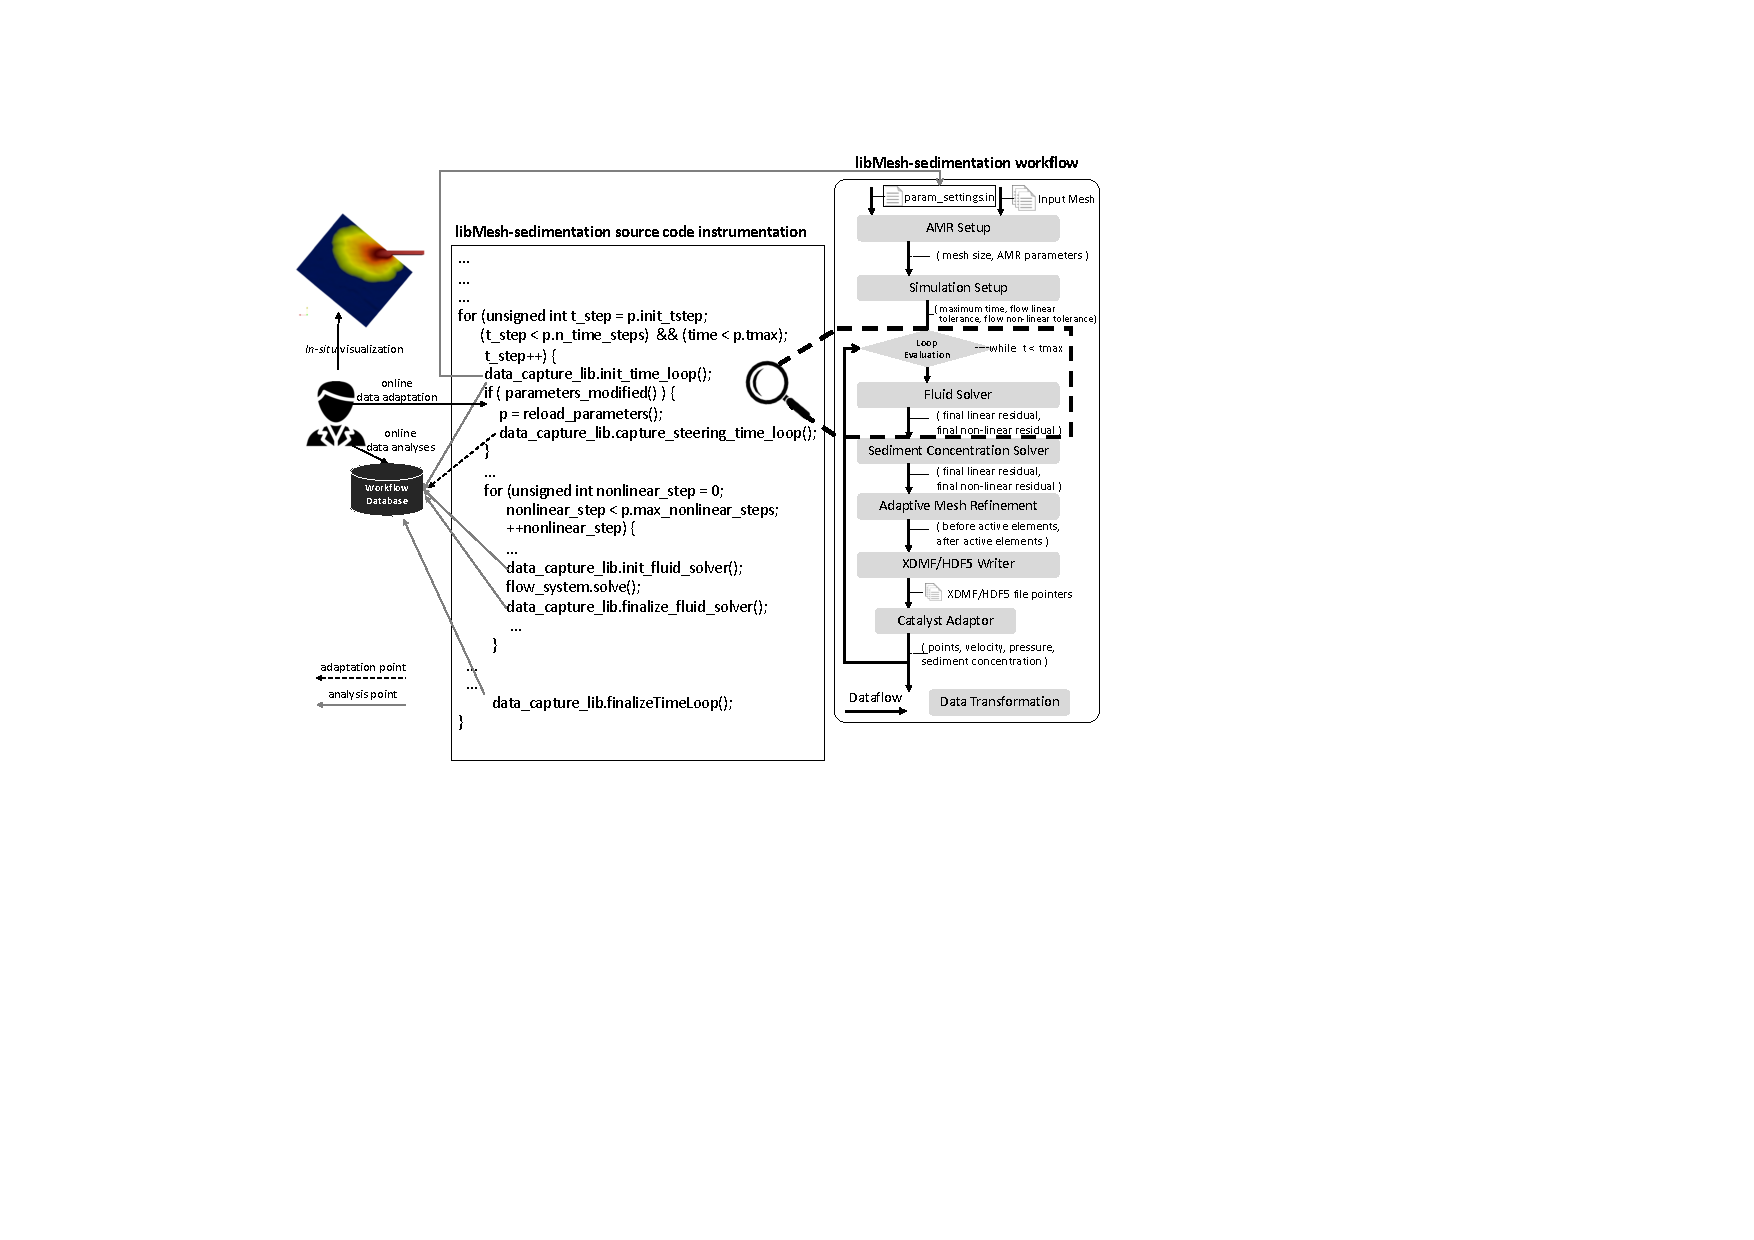
\includegraphics[width=\textwidth,keepaspectratio]{img/libmesh-experiment.pdf}
    \caption{libMesh-sedimentation workflow script code with added API calls along with its  workflow representation.}
    \label{fig:libmesh_sed_cppode}
\end{figure}



\textbf{HPC Environment and Deployment}. The experiments in this section were conducted on Lobo Carneirno cluster\footnote{http://www.nacad.ufrj.br/recursos/sgiicex}, an SGI ICE X with 252 nodes, each with a 24-core processor and 64 GB RAM, summing 6,048 cores and 16 TB RAM. The nodes are interconnected via FDR InfiniBand and share a Lustre file system with 500 TB. The Data Management services and MonetDB are deployed on a separate node in the cluster, different from the ones used by the main computational process for libMesh-sedimentation.
libMesh-sedimentation is implemented in C++ and its code with instrumentation for analysis and steering is available on GitHub \cite{libMeshSed_github} along with with DfAdapter's code \cite{DfAdapterGitHubDfAdapter}.





%%%%%%%%%%%%%%%%%%%%%%%%%%%%%%%%%%%%%%%%%%%%%%%%%%%%%%%
%%%%%%%%%%%%%%%%%%%%%%%%%%%%%%%%%%%%%%%%%%%%%%%%%%%%%%%
%%%%%%%%%%%%%%%%%%%%%%%%%%%%%%%%%%%%%%%%%%%%%%%%%%%%%%%
%%%%%%%%%%%%%%%%%%%%%%%%%%%%%%%%%%%%%%%%%%%%%%%%%%%%%%%
%%%%%%%%%%%%%%%%%%%%%%%%%%%%%%%%%%%%%%%%%%%%%%%%%%%%%%%





\subsection{User Steering Action Data Analysis}
\label{sec_steering_action_analysis_workflow_script}

\subsubsection{Small-scale case}
\label{sub_dfadapter_experiments}


The small-scale experiment is used by scientists as a benchmark to
evaluate sedimentation solvers. It simulates the laboratory test carried
out by \citet{DeRooij2001Time-} with a
lock-exchange configuration. The objective of this experiment is to show
the data analytical potential of our solution, how we record structured
parameter-tunings, and how users can query the steering action data to
enhance their analyses.

The computational setup used in this test case consists of a plane
channel with dimensions $20 * 2$ filled with sediments in suspension and
clear fluid at rest. In the laboratory, a lock-gate is used to separate
the fluids before the beginning of the experiment. When the gate is
removed, a mutual intrusion flow develops in which the particle-laden
front travels along the bottom to the right. In this simulation, the
lock-gate is located at $x = 0.75$. The non-dimensional parameters used
are $Grashof \text{ } number = \num{5.0e-6}$, $Schmidt \ number = 1.0$,
and $Settling \text{ } velocity = 0.02$. Adaptive mesh refinement is used to track
the interface between sediments concentration and clear water. Figure \ref{fig:2dtanks}
shows the concentration of sediments in suspension and the adapted mesh
at simulation time $t = 10$.

\begin{figure}[H]
    \centering
    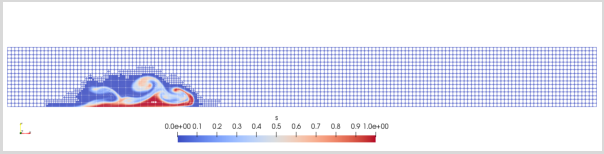
\includegraphics[width=\textwidth,keepaspectratio]{img/tank2d.pdf}
    \caption{2D visualization of the tank and the concentration of sediments. This figure was generated at simulation time $t = 10$.}
    \label{fig:2dtanks}
\end{figure}

In this simulation, the user is interested in analyzing possible performance gains when the number of nonlinear and linear (in this case, GMRES) iterations is tuned at runtime. Specific fine-tunings on different input parameters may impact the solvers and hence the simulation time considerably. During the execution, the user submits analytical queries. Based on the analyses of nonlinear and GMRES iterations, the user decides to fine-tune the solver’s parameters. In total, the user chooses to do six fine-tunings in 10 hours of simulation. Figure \ref{fig:q1steering} shows a query
that tracks the steering action. The query lists the parameters tuned by a user (say, Bob), correlated to the time steps. By running this query, other researchers are aware that Bob adapted this workflow execution six times. The times and values are well-structured and recorded in the workflow database.

\begin{figure}[H]
    \centering
    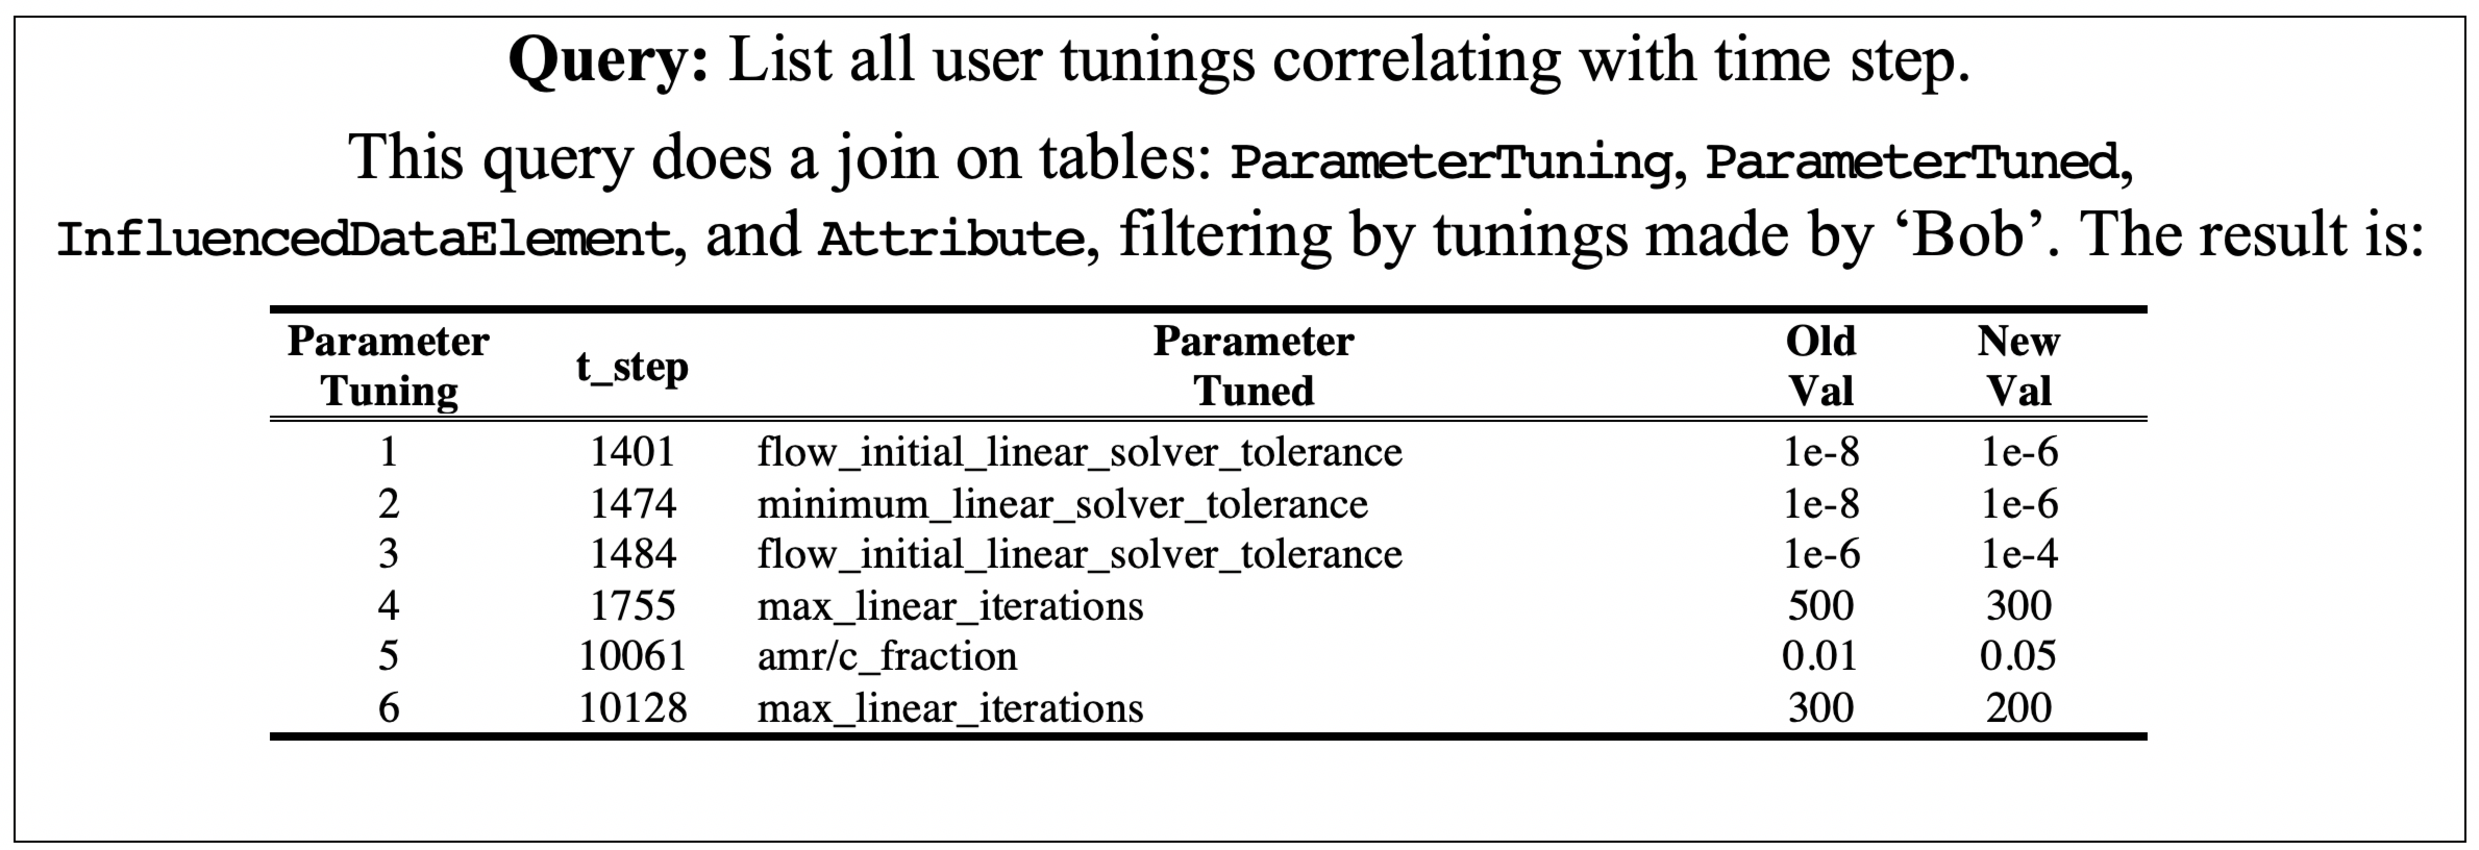
\includegraphics[width=\textwidth,keepaspectratio]{img/param_tun_q1.pdf}
    \caption{Query analyzing the track of the steering actions.}
    \label{fig:q1steering}
\end{figure}



To inspect the consequences of adaptations, a more sophisticated
analytical query is needed. Figure \ref{fig:q2steering} shows the query results
of the average values of strategic quantities ten iterations before and after each of the  fine-tunings. The results include nonlinear and linear (GMRES)
iterations, which are output values of the solver, and the number of
finite elements, which is an output of the mesh refinement process and
depends on other inputs of the solver. This query shows an integration
of provenance, domain, and execution data, and the new steering action data we introduced.

\begin{figure}[H]
    \centering
    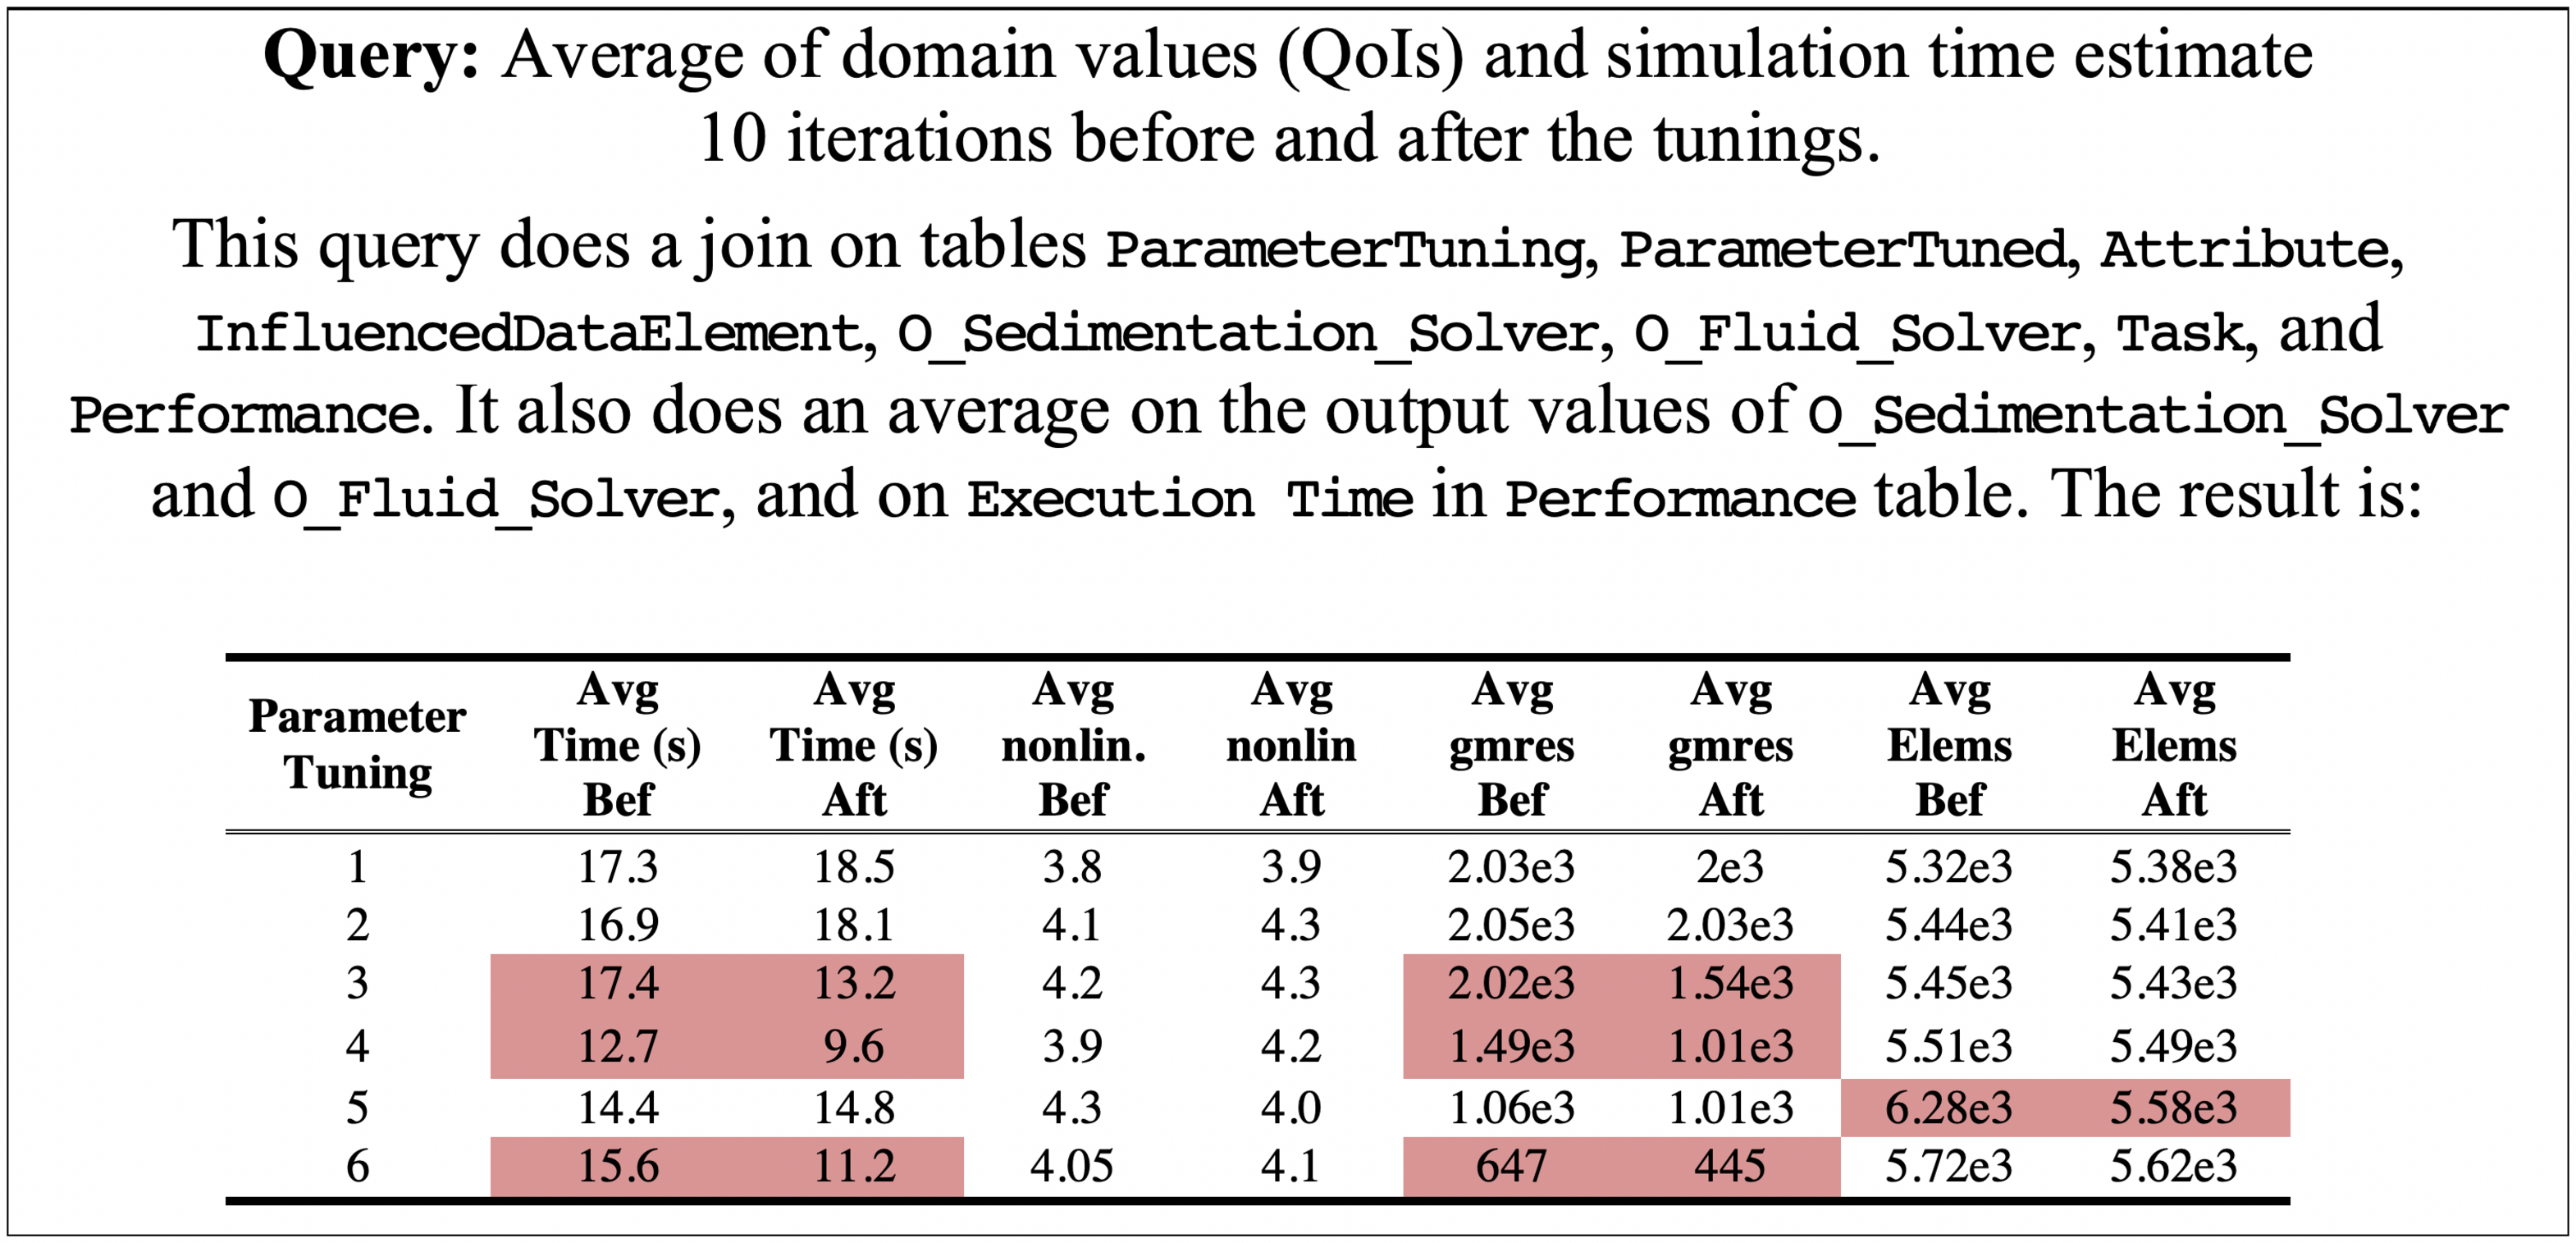
\includegraphics[width=\textwidth,keepaspectratio]{img/param_tun_q2.pdf}
    \caption{Query integrating execution, domain, provenance, and steering action data.}
    \label{fig:q2steering}
\end{figure}

The results in Figure \ref{fig:q2steering} (we highlight the main findings)
show that the Tunes \#3, \#4, and \#6 impacted the average elapsed time
and the average number of GMRES iterations, which are of high interest
to the user. Tune \#5 barely changed the other values but reduced the
number of mesh elements by about 11.15\%. This reduction is important
because when there are too many elements, out-of-memory errors may
happen (see the large-scale case next). In Figure \ref{fig:sixtunings}, we plot the evolution of
these variables over time and annotate the tunings (Tune \#1 to Tune
\#6) so the user can evaluate the adaptations.


\begin{figure}
    \centering
    \includegraphics[width=\textwidth,keepaspectratio]{img/tunes-1-to-6.png}
    \caption{Plots of monitoring queries for number of GMRES iterations, non-linear iterations, and mesh elements over time. We highlight the tune actions.}
    \label{fig:sixtunings}
\end{figure}


Based on the online analyses of user steering action data, the user
 decides whether new tunes are needed. Moreover, considering a scenario where another research team
analyzes the provenance of the results, the team sees the abrupt changes in
the results and can correlate these results with Bob's steering actions
through SQL queries in the workflow database. They can check if sudden
changes are related to one of the adaptations Bob did. Thus, they will
have a better understanding of the results.

\subsubsection{Large-scale case}

In a large-scale experiment, the user sets up the libMesh-sedimentation
workflow with a simulation of the deposition of sediments carried by a
turbidity current over a real experimental channel. A mixture of
sediments is continuously injected into a channel that deposits
sediments in the tank. The tank has $length = 135$, $width = 40$, and $height
= 50$ (dimensionless units).

The dimensionless simulation parameters are $Settling \text{ }  velocity =
\num{5.36e-6}$, $Grashof \text{ }  number =
\num{3.42e7}$, $Schmidt \text{ }  number = 1.0$, and fixed $time \text{ }  step =
0.01$.
It uses a 3D simulation with a spatial discretization using an
initial unstructured mesh with 1.2 million tetrahedra. AMR/C is employed
and three levels of uniform refinement are applied before the time loop.
The user specifies input parameter values for the sedimentation solver
(\ie{} linear and non-linear tolerances, the maximum number of linear
iterations, tolerances for AMR/C error estimation and refinement and
coarsening fractions) aiming at attaining a high-fidelity simulation.
One strategic simulation data that quantifies such level of detail is
the number of elements obtained in the mesh refinement data
transformation (the second one in the time loop). Although a large number of
elements in the mesh means a high level of detail, it also means more
memory and time consumed by the simulation. Depending on the parameter
values specified for the solver, the simulation may run out of memory.
Thus, the user does not know beforehand which range of parameters is
best for a good level of detail with acceptable memory consumption.

To support the user in following the evolution of strategic values, we
use our monitoring approach by setting up queries to the workflow database at specified time intervals (each simulation's time step). One query shows
linear and nonlinear iterations, residual norms, and the number of
elements in the mesh at each time step. Additionally, ParaView Catalyst
is set up to plot 3D visualizations of the channel and the sediment
deposits over time. Then, the user sees, for example, that the number of
elements generated by the AMR/C is close to a maximum preset number of
elements. At that rate, the simulation may crash, running out of memory.
The user knows that by changing some of the solver parameters, the
number of elements tends to decrease. Thus, the user issues a command to
adapt the solver parameters and DfAdapter automatically tracks and
registers this tuning.



In Figure \ref{fig:monitoring_plot}, we show the plot of the monitoring query for the number of
elements. We see how the number is increasing when the user decided to
fine-tune the input parameters online aiming at reducing the number of
elements. This action prevented the simulation to result in an
out-of-memory error, which would interrupt the simulation, requiring
offline tunings and job resubmission to the HPC machine.

\begin{figure}[H]
    \centering
    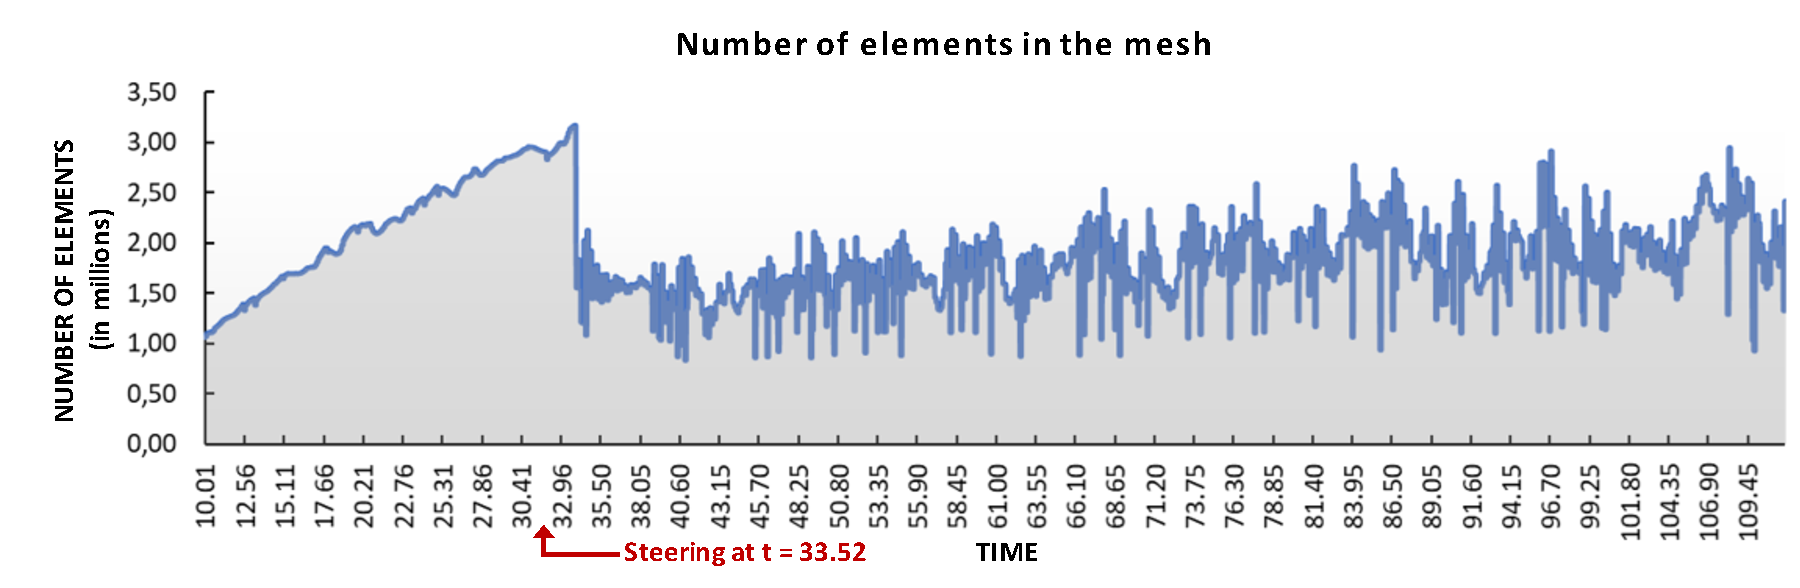
\includegraphics[width=\textwidth,keepaspectratio]{img/tuning-at-time.pdf}
    \caption{Plot of monitoring query showing number of elements over time.}
    \label{fig:monitoring_plot}
\end{figure}


 In Figure \ref{fig:largescale},
we show the 3D visualizations and the evolution of the strategic values
and how the sediments flow in the channel over time. Then, the user can
run analytical queries to analyze the consequences of the fine-tunings,
like the queries in Figures \ref{fig:q1steering} and \ref{fig:q2steering}.

\begin{figure}
    \centering
    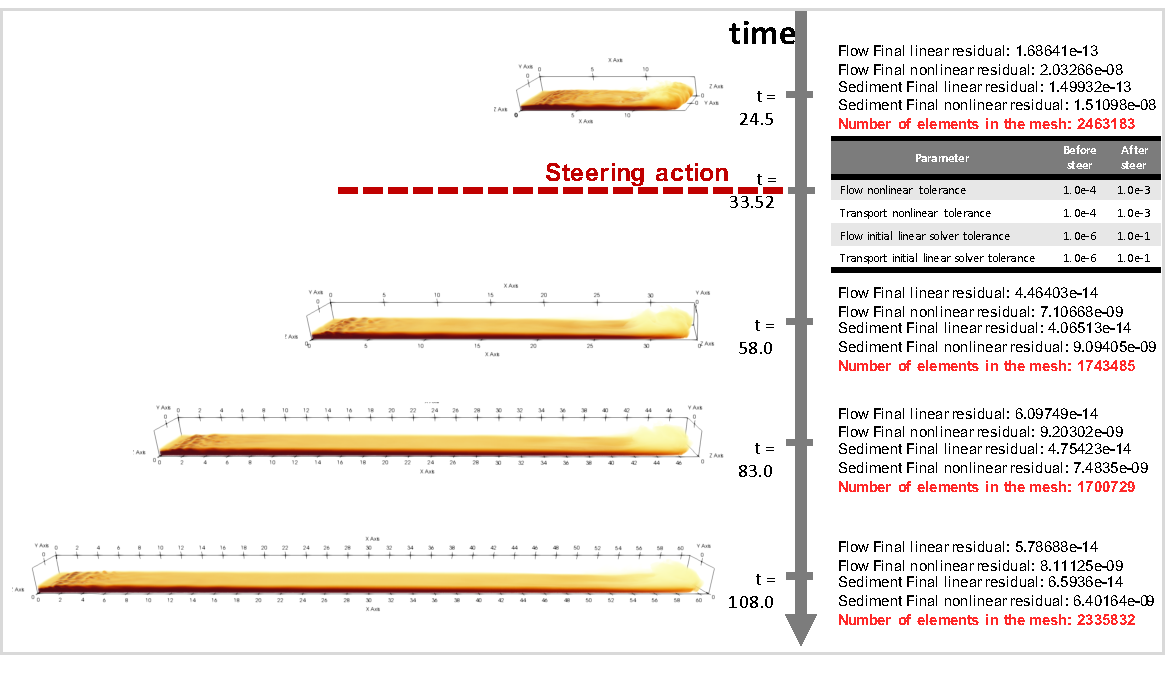
\includegraphics[width=\textwidth,keepaspectratio]{img/large-scale.pdf}
    \caption{Snapshots of 3D visualization of the tanks and the sediments over time. Steering action occurs at $t = 33.53$ and user steering data are recorded.}
    \label{fig:largescale}
\end{figure}


 In Table \ref{tab:summary_paramter_tunings}, we show a small excerpt of these
results, where we can see that the simulation time is cut down to 17
days, thanks to the fine-tunings made by the user.
If we consider the average solver time by iteration before the fine-tunings, the simulation time would be
approximately 27 days, \ie{} a reduction of 37\%. The ability our approach
gives to the users for them to have a detailed understanding of their steering
actions and the consequences of their actions (\eg{} a reduction of about 10 days
in the total execution time) improves the users' awareness, putting them in the loop
of their simulations.
These findings contribute to validating that WfSteer allows for tracking steering actions in workflow scripts.


\begin{table}[H]
\caption{Summary of results of parameter tunings.}
\label{tab:summary_paramter_tunings}
\begin{tabular}
{
 M{.22\textwidth}
 M{.22\textwidth}
 M{.22\textwidth}
 M{.22\textwidth}
}
\Xhline{4\arrayrulewidth}
\rowcolor{TableHeaderColor}


&
\textbf{Before}
&
\textbf{After}
&
\textbf{Reduction}
 \\
\Xhline{3\arrayrulewidth}

Avg. Solver Time by iteration
&
3.82 min
&
2.21 min
&
42.14\%
\\
\hline

Avg. Number of elements
&
2.4e6
&
1.7e6
&
29.24\%
\\
\hline

Total execution time
&
(expected) $\sim27$ days
&
(real)
$\sim17$  days
&
37\%
\\
\Xhline{4\arrayrulewidth}

\end{tabular}
\end{table}









%%%%%%%%%%%%%%%%%%%%%%%%%%%%%%%%%%%%%%%%%%%%%%%%%%%%%%%
%%%%%%%%%%%%%%%%%%%%%%%%%%%%%%%%%%%%%%%%%%%%%%%%%%%%%%%
%%%%%%%%%%%%%%%%%%%%%%%%%%%%%%%%%%%%%%%%%%%%%%%%%%%%%%%
%%%%%%%%%%%%%%%%%%%%%%%%%%%%%%%%%%%%%%%%%%%%%%%%%%%%%%%
%%%%%%%%%%%%%%%%%%%%%%%%%%%%%%%%%%%%%%%%%%%%%%%%%%%%%%%









\subsection{Overhead Evaluation}
\label{sec_overhead_eval_wokflow_script}

We use the concepts and equations presented in Section \ref{overhead-analysis-section} to evaluate
the overhead added to execute DfAdapter coupled with
libMesh-sedimentation workflow.
In this experiment, the added overhead is caused by
workflow data capture, raw data extraction, adaptation capabilities, and steering action data capture.
Results are in Table \ref{tab:libmeshsed_overhead}.
To obtain them, we first calculate each overhead component per task applying the Equations \ref{eq_1} to \ref{eq_5} using DfAdapter’s logging data joining with tasks’ performance data in the workflow database.
 Finally, we sum each contribution to the overall computational time as in
Equation \ref{final_eq}.


\begin{table}[H]
\caption{
The added overhead in the analysis and adaptation points account for less than 1\%; data extraction account for 1.49\%.
}
\label{tab:libmeshsed_overhead}
\begin{tabular}{
M{.14\textwidth}
M{.45\textwidth}
M{.16\textwidth}
M{.16\textwidth}
}
\Xhline{4\arrayrulewidth}
\rowcolor{TableHeaderColor}
                                     &                                           & \textbf{Total CPU time (s)} & \textbf{Total time (\%)}       \\
\Xhline{3\arrayrulewidth}

                                     & \textbf{Application computation $comp(Df)$}          & 1,407,967.18                & 98.18\%                      \\ \Xhline{0.5\arrayrulewidth}
\multirow{2}{*}{\textbf{Analysis}}   & \textbf{Analysis points $anl_{point}(Df)$}                       & 4,259.18                    & 0.3\%                        \\
                                     & \textbf{Data extraction $ext(Df)$}                   & 21,367.60                   & 1.49\%                       \\ \Xhline{0.5\arrayrulewidth}
\multirow{2}{*}{\textbf{Adaptation}} & \textbf{Adaptation point  $adp_{point}(Df)$}       & 473.24                      & 0.03\%                         \\
                                     & \textbf{Action $action(Df)$}      & 2.44                        & 1.75e-5\%                    \\ \Xhline{0.5\arrayrulewidth}
                                     & \textbf{Total $c(Df)$}                               & 1,434,069.64                & 100\%                        \\
 \Xhline{4\arrayrulewidth}

\end{tabular}
\end{table}


For analysis, workflow data capture overhead (analysis points) account for 0.3\% caused by preparing the tuples to be sent to the Data Management services.
Since
data management services and the database system run in a separate
computing resource and sending provenance data to be stored occurs
asynchronously, the data capture overhead account only for preparing
tuples to be sent. This represents a very low overhead, in the order of
few milliseconds per task.
libMesh-sedimentation workflow has an adaptation point at the beginning of the time loop iteration.
Raw data extractors, provided by DfAnalyzer, extract convergence values from raw data files written as XDMF/HDF5 so the user can monitor and detect possible misbehavior of nonlinear and linear solvers.
Extracting data values from raw data files to store in a
database for analysis is done synchronously. Depending on the amount
of data and how the raw data extractor is implemented, overhead may not
be negligible. Here, these raw data extractions account for 1.49\% of the total computation time. For adaptation points, since libMesh-sedimentation uses a file-based checks implementation, it verifies if a file has been modified at each new time iteration. This file verification is synchronous because the workflow script must verify if a change has happened before it can continue. In total, this check at each new iteration adds 0.03\% overhead.
When a steering action happens, the internal data structure that contains the solver parameters is reloaded and steering data are captured and sent to the Data Management services. Since the user steered 6 times during the execution of this workflow, the overhead for steering action tracking is close to 0\%.

Besides, as a CSE application, in libMesh-sedimentation, tasks last for seconds-long on average (Figure \ref{fig:q2steering})
and the distributed CPUs spend significantly more time computing the application tasks than computing our data capture operations.
Therefore, considering approximately 17 days of total execution time (about $\num{1.4e6}$ seconds as shown in Figure \ref{fig:q2steering}), workflow data capture and steering action data capture together account for less than 1\% overhead, whereas summing with raw data extractions, the total overhead is less than 2\%.


Such reduced overhead is due to our system design principles related to asynchronicity and to the fact that the most costly data tracking operations, which give the structure and
data relationships, occur in the data management services running on a separate node in the HPC machine.
Anyhow, any overhead caused by any WfSteer implementation is greatly compensated by the benefits it makes to the user. For example, allowing for tracking the adaptations benefited reproducibility, validation, and interpretation. Also, observing at runtime that the adaptation reduced the execution time in ten days is relevant for further online tunings and result analyses.
These findings contribute to validating that WfSteer allows for managing steering action with low execution overhead in workflow scripts.
